\documentclass[titlepage]{article}

\usepackage[hidelinks]{hyperref}
\usepackage[table]{xcolor}
\usepackage[english]{babel}
\usepackage{tabularx}
\usepackage[toc,page]{appendix}
\setcounter{secnumdepth}{5}
\usepackage{tikz}
\usepackage{enumitem}
\usepackage{pdfpages}
\usepackage{graphicx}
\usepackage{indentfirst} 

%
\usetikzlibrary{arrows, trees, positioning, fit, calc, shadows.blur, shapes.symbols}

\usepackage[top=1.5in, bottom=1.5in, left=2in, right=2in]{geometry}

\def\getfirstword#1{%
    \begingroup
    \edef\@tempa{#1\space}%
    \expandafter\endgroup
    \expandafter\readwords\@tempa\relax
}
\def\readwords#1 #2\relax{%
      \doword{#1}%  #1 = substr, #2 = rest of string
}
\def\doword#1{#1}
\def\endtestwords{}

\newcommand{\myparagraph}[1]{\paragraph{#1}\mbox{}\\}

\addtolength{\oddsidemargin}{-.875in}
\addtolength{\evensidemargin}{-.875in}
\addtolength{\textwidth}{1.75in}

\def \TACS {Track and Control System}

\begin{document}

\title{
\textbf{
Software Design Description}
\protect\\
for the
\protect\\
\textbf{
Track and Control System}
\protect\\
{\small Version 1.0}}

\author{Robert Moss, Aaron Periera, Matthew Shrago}
\maketitle

\newpage
\tableofcontents{} 
\newpage

\section{Introduction}

\subsection{Purpose}
The Software Design Document (SDD) is intended to describe the software components of the Track and Control System (TACS). The SDD will include details about the software implementation, the database handling, and the overall design. 

\subsection{Scope}
\begin{enumerate}
	\item The software will track a user's movements and be able to control numerous features around their Desktop with the movement of their head.
	\begin{itemize}	 	 	
  	\item The everyday computer user will utilize this software to organize their cluttered Desktop.  	
	\end{itemize}
  	\item The application will also act as a security monitor to recognize when you're present at your computer and lock your screen accordingly.
  	\begin{itemize}
  		\item A benefit of this will be a sense of security for the user when they're away from their computer.
  	\end{itemize}
  \end{enumerate} 

\subsection{Overview}
The SDD will contain explicit details about the TACS software. Distinct acronyms and definitions will be clarified. References for our specified libraries will be included. A system overview of the software architectural design as well as the database design will be covered. Finally, the proposed interface design will also be established and talked about. 

\subsection{Reference Material}
The list of references below are software documentation that we will be using:
\begin{enumerate}
	\item OpenCV documentation: \href{http://opencv.org/}{\color{blue} http://opencv.org/}
	\begin{itemize}
		\item FaceRecognizer API: \href{http://docs.opencv.org/trunk/modules/contrib/doc/facerec/facerec\_api.html}{\color{blue} http://docs.opencv.org/trunk/modules/contrib/doc/facerec/facerec\_api.html}
	\end{itemize}
	\item Windows API Index: \href{http://msdn.microsoft.com/en-us/library/hh920508(v=vs.85).aspx}{\color{blue} http://msdn.microsoft.com/en-us/library/hh920508(v=vs.85).aspx}
	\item QT C++ documentation: \href{http://qt-project.org/}{\color{blue} http://qt-project.org/}
\end{enumerate}

\subsection{Definitions, Acronyms, and Abbreviations}
\begin{itemize}
	\item Application Specific Definitions
	\begin{itemize}
		\item TACS - Track and Control System
		\item TM - Tracking Module
		\begin{itemize}
			\item OT - Object Tracker
			\item FRT - Facial Recognition Tracker
		\end{itemize}
		\item WCM - Windows Control Module
		\begin{itemize}
			\item WGO - Windows Grid Organizer
			\item WP - Windows Perspective
		\end{itemize}
		\item SM - Settings Module
	\end{itemize}
	\item Industry Definitions
	\begin{itemize}
		\item SRS - Software Requirements Specification
		\item OpenCV - Open Computer Vision: An open source library for object tracking via the camera.
		\item SQLite - A lightweight, low maintenance, self contained local database.
		\item DB - Database
		\item RGB - Red, Green, Blue color values.
		\item HSV - Hue, Saturation, Value.
		\item API - Application Programming Interface
		\item C++ - An object oriented programming language.
		\item GUI - Graphical User Interface
		\item QT - An API for building GUIs
	\end{itemize}
\end{itemize}

\section{System Overview}
There will be many available functions the users can utilize. The modular design of the software will allow for additional functions to be easily implemented. \textit{It should be noted that the window functions will be activated with a user-defined hot key.}
\begin{enumerate}
	\item A proportional snap to grid set up for users to place desired windows in five different locations. Namely, left, right, top, bottom, and middle. Once all the windows are selected, the middle window will fill the screen and the user will be able to "peer" in the direction of the four other windows to show a preview of them. 
	\item The software will organize all open windows into a layered view (with the illusion of 3D windows) for the user to "look" around their desktop and see which window they want to select.
	\item The software will be able to detect when the user is away from the screen, and with a user defined delay-time, be able to lock or put your computer to sleep (all settings can be changed from the SM).
\end{enumerate}

\section{System Architecture}
% Architectural Design
\includepdf[clip,trim=0mm 75mm 0mm 0mm,pagecommand=\subsection{Architectural Design}]{architectural_design.pdf}

% Decomposition Description
\includepdf[scale=0.75,pagecommand=\subsection{Decomposition Description}]{decomposition_description.pdf}

\subsection{Design Rationale}
The design is highly modular. The justification for this is because there are several different ways to complete the tasks at hand. Tracking the user can be done in numerous ways, as long as it follows the TrackingModule interface and outputs the set of $x$ and $y$ coordinates. This is the same for the WindowsControlModule. New features can be added into the system due to the modularity. As long as the new feature follows the output data structure that the others obey, it can be easily incorporated into TACS. The SettingsModule is completely separate from the main functionality of TACS; allowing it to write to the database and solely worry about that process.

\section{Data Design}
\subsection{Data Description}
There will be a data structure, defined by the developers, that will hold all the necessary data to be written to the SQLite database. The data structure will be represented in the same way as the Data Dictionary below. Most components will have settings that need to be remembered. The dictionary below outlines which component will have the specified data associated with it.

\subsection{Data Dictionary}
\begin{center}
	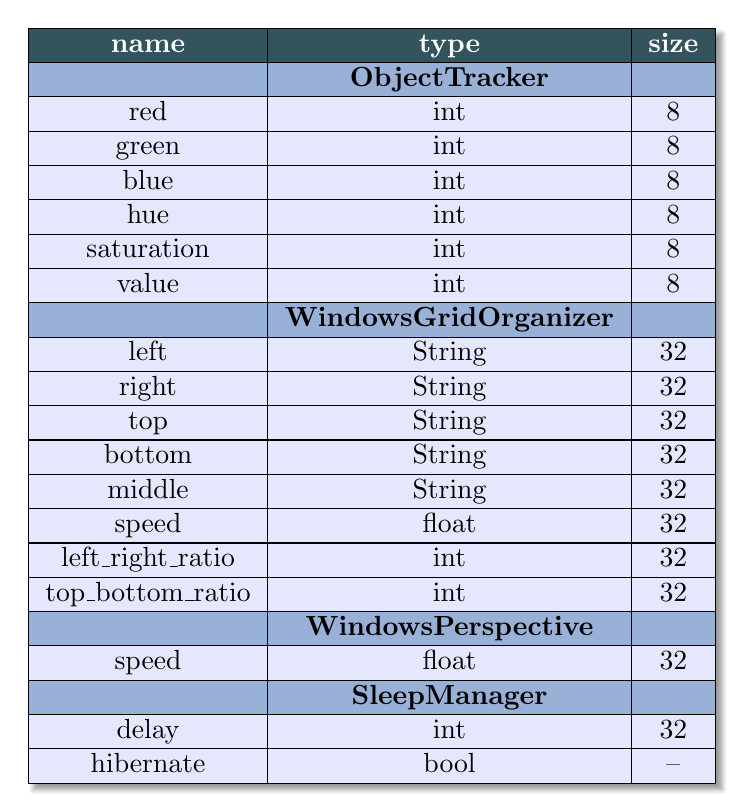
\begin{tikzpicture}
		\node[blur shadow={shadow blur steps=5},fill=white,inner sep=0pt] 
		{\rowcolors{1}{black!10!green!10!blue!10}{black!10!green!10!blue!10}
		\centering
		\begin{tabular}{ | c | c | c | }
		\hline
		\rowcolor{black!80!green!80!blue!80} {\color{white} \textbf{name}} & {\color{white} \textbf{type}} & {\color{white} \textbf{size}} \\
		\hline
		\rowcolor{black!40!green!40!blue!40} & \textbf{ObjectTracker} & \\
		\hline
		red & int & 8 \\
		\hline
		green & int & 8 \\
		\hline
		blue & int & 8 \\
		\hline
		hue & int & 8 \\
		\hline
		saturation & int & 8 \\
		\hline
		value & int & 8 \\
		\hline
		\rowcolor{black!40!green!40!blue!40} & \textbf{WindowsGridOrganizer} & \\
		\hline
		left & String & 32 \\
		\hline
		right & String & 32 \\
		\hline
		top & String & 32 \\
		\hline
		bottom & String & 32 \\
		\hline
		middle & String & 32 \\
		\hline
		speed & float & 32 \\
		\hline
		left\_right\_ratio & int & 32 \\
		\hline
		top\_bottom\_ratio & int & 32 \\
		\hline
		\rowcolor{black!40!green!40!blue!40} & \textbf{WindowsPerspective} & \\
		\hline
		speed & float & 32 \\
		\hline
		\rowcolor{black!40!green!40!blue!40} & \textbf{SleepManager} & \\
		\hline
		delay & int & 32 \\
		\hline
		hibernate & bool & -- \\
		\hline
		\end{tabular}
		};
	\end{tikzpicture}
\end{center}

\section{Component Design}
\subsection{TrackingModule}
The TrackingModule will be the supper-class for the ObjectTracker, FacialRecognitionTracker, and MouseTracker. Each sub-class will hold the $x$ and $y$ values of the tracked user. The $track()$ function will be implemented differently for each sub-class. The ObjectTracker will need the RGB or the HSV values set by the user. The FRT won't need any extra variables, as it will recognize any face, not a specific face. Lastly, the MouseTracker will simply track the coordinates of the mouse and send them out as the $x$ and $y$ outputs.

\subsection{WindowsControlModule}
The WCM will act as a super-class for the WindowsGridOrganizer, WindowsPerspective, and SleepManager. All sub-classes will have the DataStruct, \textit{settings}, to be updated and set out as output. The WGO will keep track of which window was selected for each grid section in a String array. Then it will set the grid positioning with $setGrid()$. The WP will gather all the open windows to be resized and projected. The SleepManager will run the $sleep()$ function with the user defined delay (defaulted to a specified value). Each sub-class will output the DataStruct directly to the SettingsModule. 

\subsection{SettingsModule}
The SettingsModule will write the inputted DataStruct to the local SQLite database. Default values will be handled here.

\section{Human Interface Design}
\subsection{Overview of User Interface}
The GUI will be very minimal, seeing as most of the software features will utilize the open windows. A tabbed view of the Tracking options and the Windows Control option will be present. 

Within the Tracking tab, the user will be able to change the settings for which tracking method they prefer. They will also be able to see the camera and how it's tracking. 

The Windows Control tab will have a list of available features. When clicking on an item in this list, the user will have the options for that feature presented to them. Keeping each features options separated in the list will enable the addition of features to be easily implemented. 

\subsection{Screen Images}
\subsubsection{Tracking Tab}
\includegraphics[scale=0.8]{gui/tracking_tab.png}

\subsubsection{Windows Control Tab}
\includegraphics[scale=0.8]{gui/windows_control_tab.png}

\subsection{Screen Objects and Actions}
Only one tracking method can be selected at a time. The settings for that method will appear to the right when it's selected (Object Tracking shown).

The Windows Control tab will include the list of features. The spinners for the Left/Right Width and Top/Bottom Height will be a percentage from 0-100 of the screen width and height, respectively.

\newpage
\section{Requirements Matrix}
\begin{center}
\begin{table}[h]
	\centering
	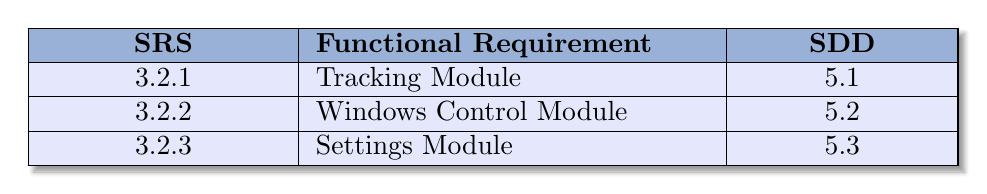
\begin{tikzpicture}
	\node[blur shadow={shadow blur steps=5},fill=white,inner sep=0pt] 
	{\rowcolors{1}{black!40!green!40!blue!40}{black!10!green!10!blue!10}
		\begin{tabular}{ | >{\centering}p{3cm} | p{5cm} | >{\centering\arraybackslash}m{2.5cm} |}
		\hline
		\textbf{SRS} & \textbf{Functional Requirement} & \textbf{SDD} \\
		\hline
		3.2.1 & Tracking Module & 5.1 \\
		\hline
		
		\rowcolor{black!10!green!10!blue!10}3.2.2 & Windows Control Module & 5.2 \\
		\hline
		3.2.3 & Settings Module & 5.3 \\
		\hline
		\end{tabular}
	};
	\end{tikzpicture}
\end{table}
\end{center}


\end{document}